%!TEX root = ../NCVC5.tex

\mysection{複数のCADデータを統合}

\subsection{CADデータの統合からNCプログラムの生成まで}
 加工したいCADデータが複数あって,それを大きなワークエリアから切り出したいとき,1つずつ加工するには原点を再調整しなければならないなど操作が面倒です.
CADデータの段階で簡単に併合できれば良いのですが,そういうことを想定して作られていないせいか意外と面倒だったりします.
また数が多いとその操作も大変でしょう.
\begin{center}
\textbf{NCVCで簡単に統合できるようになりました~!!}
\end{center}
 \menu{ファイル>CADデータの統合} を選択すると図\ref{fig:bind.png} のダイアログが出てきます.

\begin{figure}[H]
\centering
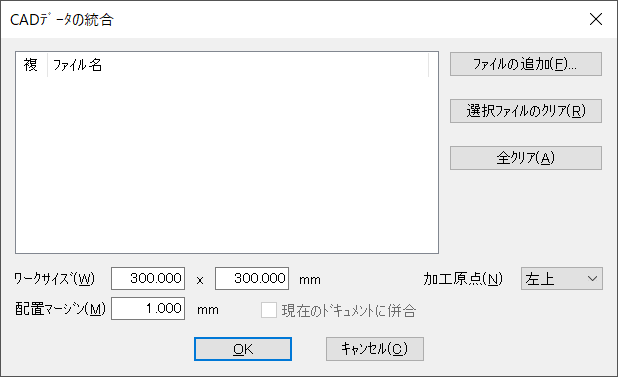
\includegraphics[scale=0.7]{No1/fig/bind.png}
\caption{CADデータの統合ダイアログ}
\label{fig:bind.png}
\end{figure}

 [ファイルの追加]ボタンを押してCADデータを追加してください.
読み込めるファイル形式は,アドインでサポートされているデータ形式を含むCADデータです.
JWW形式やDXF形式を混在させることも可能です.
ファイルは \keys{SHIFT}や\keys{CTRL}キーを押しながらの複数選択が可能です.
このダイアログにD\&Dすることも可能です.
追加されたファイルの[複]の欄に2以上の数値を入れるとその分複製されます.
ワークサイズは貼り付ける領域を指定し,配置マージンはCADデータを配置するときのすき間を指定します.
[現在のドキュメントに併合]チェックボックスは,現在NCVCで開いているドキュメントが統合後ドキュメントのときアクティブになり,そのドキュメントに追加したい場合にチェックを入れます.

 ファイルの選択が終われば,OKボタンを押してください.
図\ref{fig:sample1.png} のように指定されたワーク矩形の中にCADデータが配置されます.
配置はNext-Fit Algorithm(NF法)と呼ばれるアルゴリズムをベースに少し改良を加えています.
詳しくは『長方形 詰め込み』等で検索してみてください.

\begin{figure}[H]
\centering
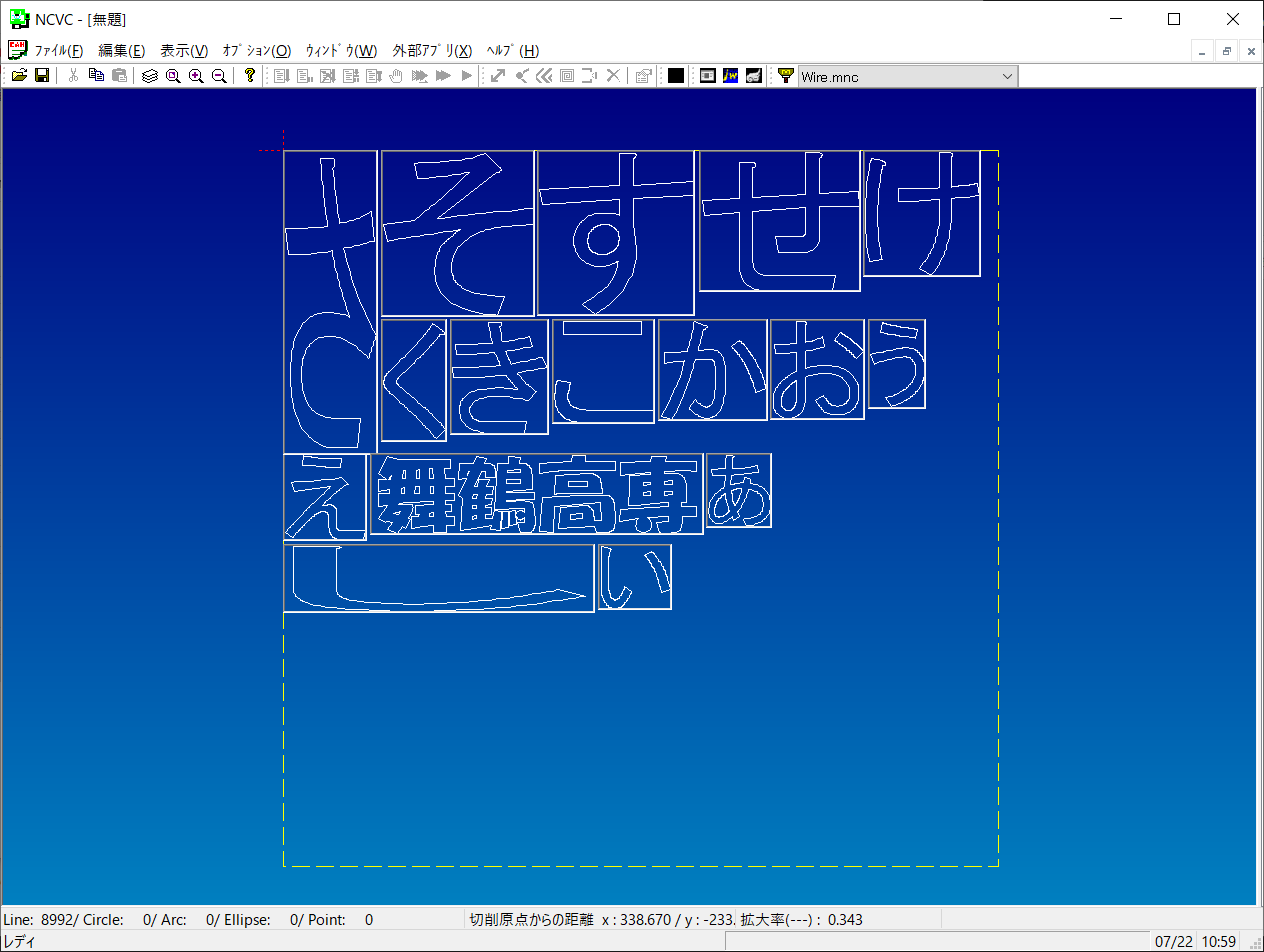
\includegraphics[scale=0.5]{No1/fig/sample1.png}
\caption{NF法によるCADデータの配置}
\label{fig:sample1.png}
\end{figure}

 凹型と凸型をうまく組み合わせるようなことはしません.
データの最大矩形で配置されます.
しかも若干おバカさんなので人間がうまくフォローしてあげてください.
操作方法は表\ref{tab:key} のようになっています.
ほぼWindowsで行う通常操作に準拠して作られています.

\begin{table}[H]
\centering
\caption{操作方法}
\label{tab:key}
\begin{tabular}{|l|l|}
\hline
左クリック & 選択の切り替え \\
  \keys{CTRL}押しながら & 複数の選択 \\ \hline
左ドラッグ & 配置の移動 \\
  \keys{SHIFT}押しながら & 水平垂直の移動 \\
  移動中の\keys{ESC}または右クリック & 移動キャンセル \\ \hline
配置外からの左ドラッグ & 範囲選択 \\ \hline
右ドラッグ & パン(従来通り)\\ \hline
\keys{CTRL+Z} & 移動を元に戻す \\ \hline
左ダブルクリック & 左90度回転 \\ \hline
\keys{SHIFT}+左ダブルクリック & 右90度回転 \\ \hline
右クリック(ポップアップメニュー) & 処理対象の切り替え \\ \hline
\keys{SHIFT+DEL} & 削除(UNDO不可)\\ \hline
\end{tabular}
\end{table}

 移動について少しだけ注意が必要です.
内部計算(論理座標)では精度よく配置されていますが,マウスで移動させるとピクセルから論理座標への変換で若干の誤差が出ます.
配置原点だけでCADデータの中身には影響がないのでご安心ください.
配置さえも正確に行いたい場合は,面倒ですがCADソフトで配置させてください.
後述しますが,この状態でDXFへの出力が可能です.

 [処理対象の切り替え]は,NC生成やDXF出力に対して一時的に対象外とする場合に使用します.
加工を途中から再開したい場合などに使えると思います.

\begin{figure}[H]
\centering
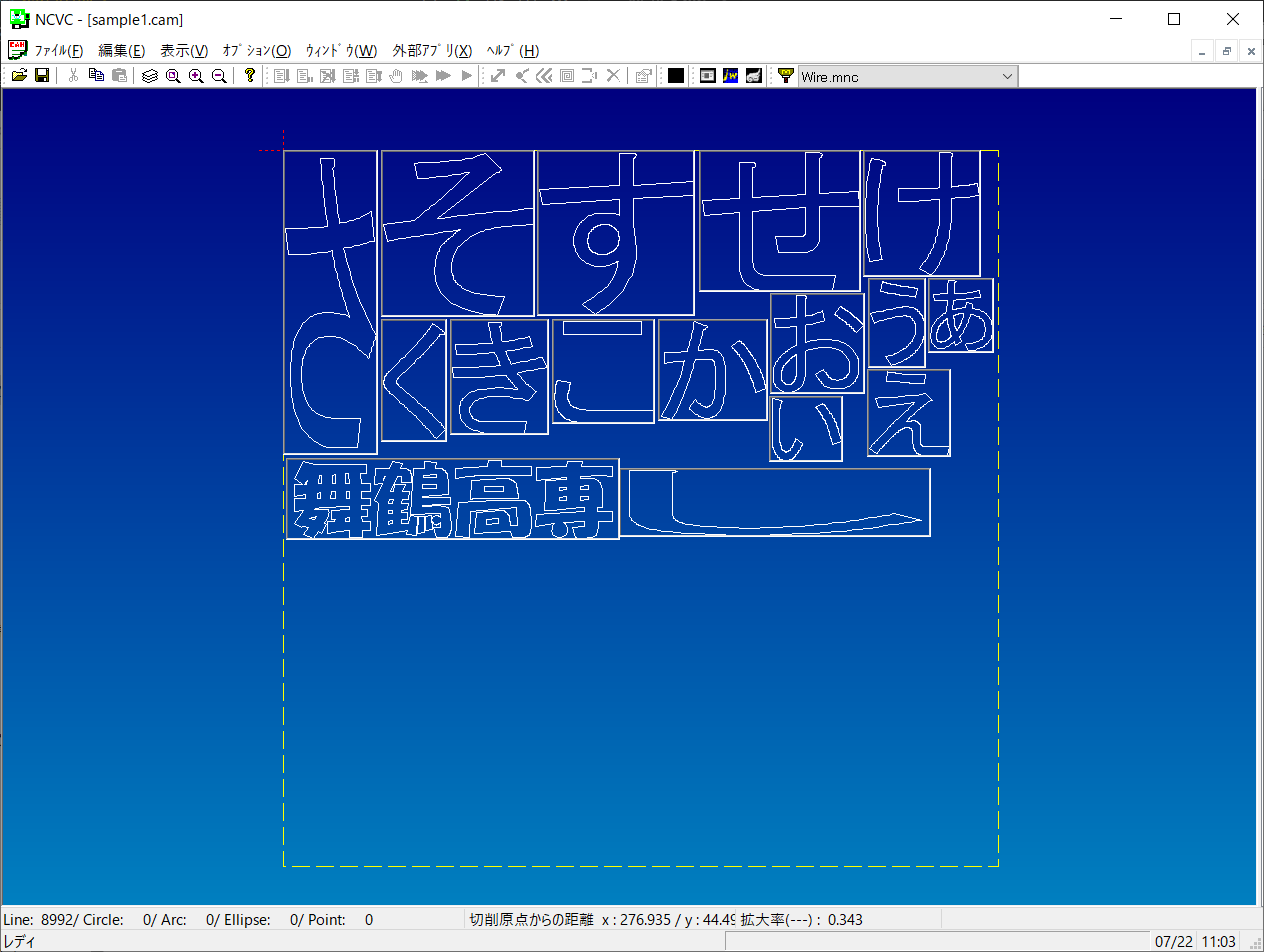
\includegraphics[scale=0.5]{No1/fig/sample2.png}
\caption{自動配置から若干の手直し}
\label{fig:sample2.png}
\end{figure}

 あとは通常の工程でNCプログラムが生成可能です.
条件(レイヤが2つ以下)さえ整っていればワイヤ放電加工機用のデータも生成可能です.

\begin{figure}[H]
\centering
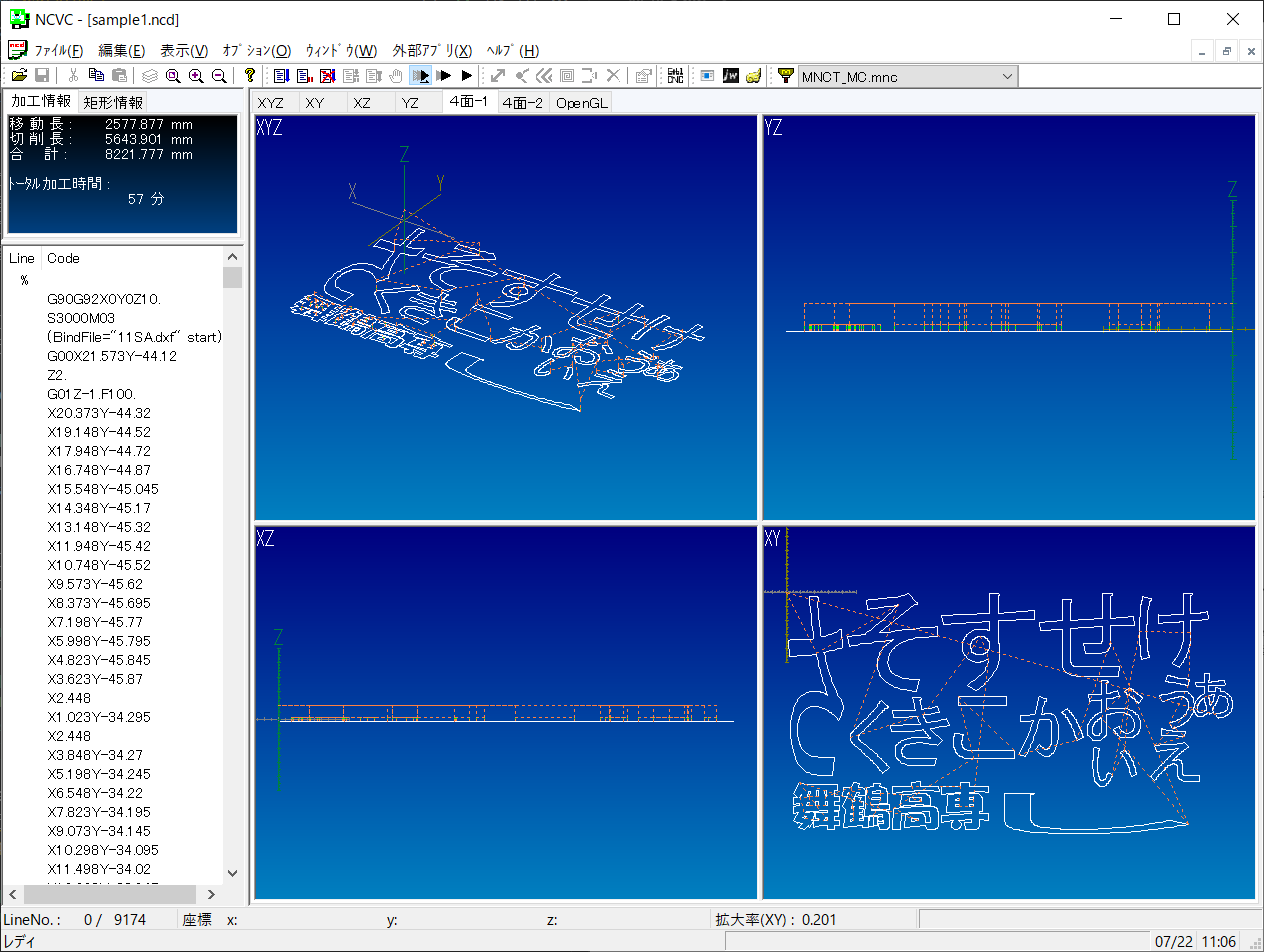
\includegraphics[scale=0.5]{No1/fig/simu1.png}
\caption{生成されたNCプログラム}
\label{fig:simu1.png}
\end{figure}

\subsection{統合生成オプション}
 統合状態からNCプログラムの生成を行うと,図\ref{fig:option1.png} の[統合時オプション]ボタンが表示されます.
図\ref{fig:option2.png} のオプションが設定可能なので,状況に合わせて設定してあげてください.

\begin{minipage}[t]{0.5\textwidth}
\begin{figure}[H]
\centering
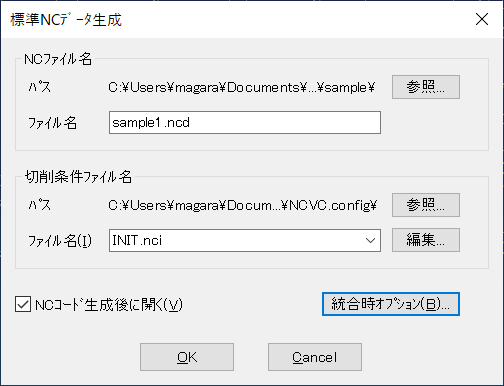
\includegraphics[scale=0.7]{No1/fig/option1.png}
\caption{NCデータ生成ダイアログ}
\label{fig:option1.png}
\end{figure}
\end{minipage}
\begin{minipage}[t]{0.5\textwidth}
\begin{figure}[H]
\centering
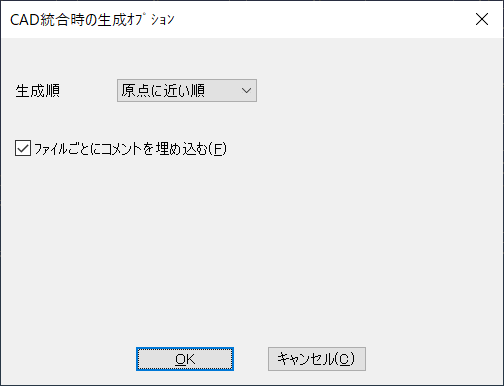
\includegraphics[scale=0.7]{No1/fig/option2.png}
\caption{統合生成オプション}
\label{fig:option2.png}
\end{figure}
\end{minipage}

\vspace*{2zh}
 [ファイルごとにコメントを埋め込む]オプションを有効にすると,
NCプログラム内に(BindFile=``\,\textit{filename}\,'' start)とコメントが埋め込まれます.
エディタ編集時に活用してください.
ただし,漢字のファイル名には要注意です.
加工機側で不具合が生じる可能性があります.
